\part{Tinkering Graphics}
\frame{\partpage}

\begin{frame}
	\frametitle{Light Perception}
	\begin{itemize}
		\item Colour is continuous:
		\begin{itemize}
			\item Visible light is in the wavelengths between 370nm and 730nm
			\item i.e., 0.00000037 --- 0.00000073 meters
		\end{itemize}
		\item However, we \textit{perceive} light around three particular peaks:
		\begin{itemize}
			\item Blue peaks around 425nm
			\item Green peaks around 550nm
			\item Red peaks around 560nm
		\end{itemize}
	\end{itemize}
\end{frame}

\begin{frame}
	\frametitle{Light Perception}
	\begin{itemize}
		\item Our eyes have three types of colour-sensitive photoreceptor cells called `cones' that respond to light wavelengths
		\item Our perception of colour is based on how much of each kind of sensor is responding
		\item An implication of this is perception overlap: we see two kinds of `orange' --- one that's spectral and one that's combinatorial
	\end{itemize}
\end{frame}

\fullbleed{1416_Color_Sensitivity}

\begin{frame}
	\frametitle{Luminance vs Colour}
	\begin{itemize}
		\item Our eyes have another type of photoreceptor cells called `rods' that respond to light intensity
		\item Our perception, however, is actually luminance: a relativistic contrast of \textit{borders} of things (i.e., motion) 
		\begin{itemize}
			\item Luminance is \textit{not} the amount of light, but our perception of the amount of light
			\item Much of our luminance perception is based on comparison to background, not raw values
		\end{itemize}
		\item An implication of this is perception overlap: we see blue as `darker' than red when the intensity is actually the same
	\end{itemize}
\end{frame}

\fullbleed{grayscale}

\begin{frame}
	\frametitle{Resolution}
	\begin{itemize}
		\item We have a limited number of rods and cones in our eyes
		\item This means humans perceive vision in a limited resolution --- yet, we perceive vision as continuous
		\item We take advantage of this human characteristic in computer monitors
	\end{itemize}
\end{frame}

\fullbleed{sony-dsc-29-625x1000}

\begin{frame}
	\frametitle{Pixels}
	\begin{itemize}
		\item We digitize pictures into many little dots
		\item Enough dots and it looks like a continuous whole to our eye
		\item Each element is referred to as a \textit{pixel}
	\end{itemize}
\end{frame}

\begin{frame}
	\frametitle{Pixels}
	
	Pixels must have:
	
	\begin{itemize}
		\item a color
		\item a position
	\end{itemize}
\end{frame}

\begin{frame}
	\frametitle{Pictures and Surfaces}
	
	In PyGame, a \texttt{Surface} is a \textit{matrix} of pixels
	
	\begin{itemize}
		\item It is not a continuous line of elements, that is, a one-dimensional \textit{array}
		\item A picture has two dimensions: width and height
		\item It's a two-dimensional \textit{array}
	\end{itemize}
\end{frame}

%\fullbleed{pic_array}

%\fullbleed{pic_matrix}

\begin{frame}
	\frametitle{Pictures and Surfaces}
	
	\begin{itemize}
		\item (x, y) ---or--- (horizontal, vertical)
		\item The origin (0,0) is top-left
		\item (1,0) = 12
		\item (0, 2) = 6
	\end{itemize}
\end{frame}

\begin{frame}
	\frametitle{Encoding Colour}
	
	\begin{itemize}
		\item Each element in the matrix is a pixel, with the matrix defining its position and the value defining  its colour
		\item Computer memory stores numbers, so colour must be encoded into a number:
		\begin{itemize}
			\item CMYK = cyan, magenta, yellow, black
			\item HSB = hue, saturation, brightness
			\item RGBA = red, green, blue, alpha (transparency)
		\end{itemize}
		\item By default, Visual Studio and C\# uses RGBA
	\end{itemize}
\end{frame}

\begin{frame}[fragile]
	\frametitle{Encoding RGB}
	
	\begin{itemize}
		\item Each component color (red, green, and blue) is encoded as a single byte
		\item Colors go from %\lstinline{(0,0,0)} to \lstinline{(255,255,255)}:
		\begin{itemize}
			\item If all three components are the same, the colour is in grey-scale
			\item  \lstinline{(0,0,0)} is black
			\item  \lstinline{(255, 255, 255)} is white
		\end{itemize}
	\end{itemize}
\end{frame}



\begin{frame}
	\frametitle{Encoding Bits}
	
	Why \texttt{255}?
	
	\begin{itemize}
		\item If we have one bit, we can represent \textbf{TWO} patterns:
		\begin{itemize}
			\item 0
			\item 1
		\end{itemize}
		
		\item If we have two bits, we can represent \textbf{FOUR} patterns:
		\begin{itemize}
			\item 00
			\item 01
			\item 10
			\item 11
		\end{itemize}
		\item With \textit{n} bits, we can have $2^n$ patterns
		\item With $8$ bits, there will be $256$ patterns
		\item One of these patterns will be $0$, so the highest value we can represent with $8$ bits is: $2^8 - 1$, or $255$
	\end{itemize}
\end{frame}
\begin{frame}
	\begin{center}
		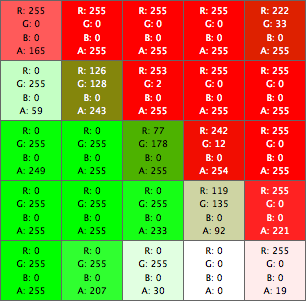
\includegraphics[scale=0.5]{rgb_pallette}
	\end{center}	
\end{frame}
\begin{frame}
	\frametitle{Encoding Bits}
	\begin{itemize}
		\item RGB uses 24-bit color (i.e., $3 * 8$ = 24)
		\begin{itemize}
			\item That's 16,777,216 possible colours
			\item Our eyes cannot discern many colours beyond this
			\item A challenge is display technology: monitors and projectors can`t reliably reproduce 16 million colours
		\end{itemize}
		\item RGBA uses 32-bit colour
		\begin{itemize}
			\item No additional colour, but offers support for transparency
			\item This transparency channel is called \texttt{alpha}
			\item The alpha channel also requires 8 bits
		\end{itemize}
		\item Assuming \texttt{1 byte} == \texttt{8 bits}
		\item We can use this information to estimate the size of a bitmap:
		\begin{itemize}
			\item 320x240x24 = 230,400 bytes
			\item 640x480x32 = 1,228,800 bytes
			\item 1024x768x32 = 3,145,728 bytes
		\end{itemize}
	\end{itemize}
\end{frame}

\fullbleed{texture-254576_1920}

\begin{frame}[fragile]
	\frametitle{Manipulating Bitmap Pixels}
	
	\begin{itemize}
		\item Images are controlled and manipulated using the \texttt{Bitmap} class in C\#
		\item We can use \texttt{GetPixel} and \texttt{SetPixel} methods to both find and change pixels.
	    \begin{lstlisting}
myImage.GetPixel(x, y);
myImage.SetPixel(x, y, newColor);
	    \end{lstlisting}
	    \item Both methods use cartesian coordinates (x and y) to define the position of a specific pixel
	\end{itemize}
\end{frame}

\begin{frame}[fragile]
	\frametitle{Manipulating Bitmap Pixels}
\begin{center}
	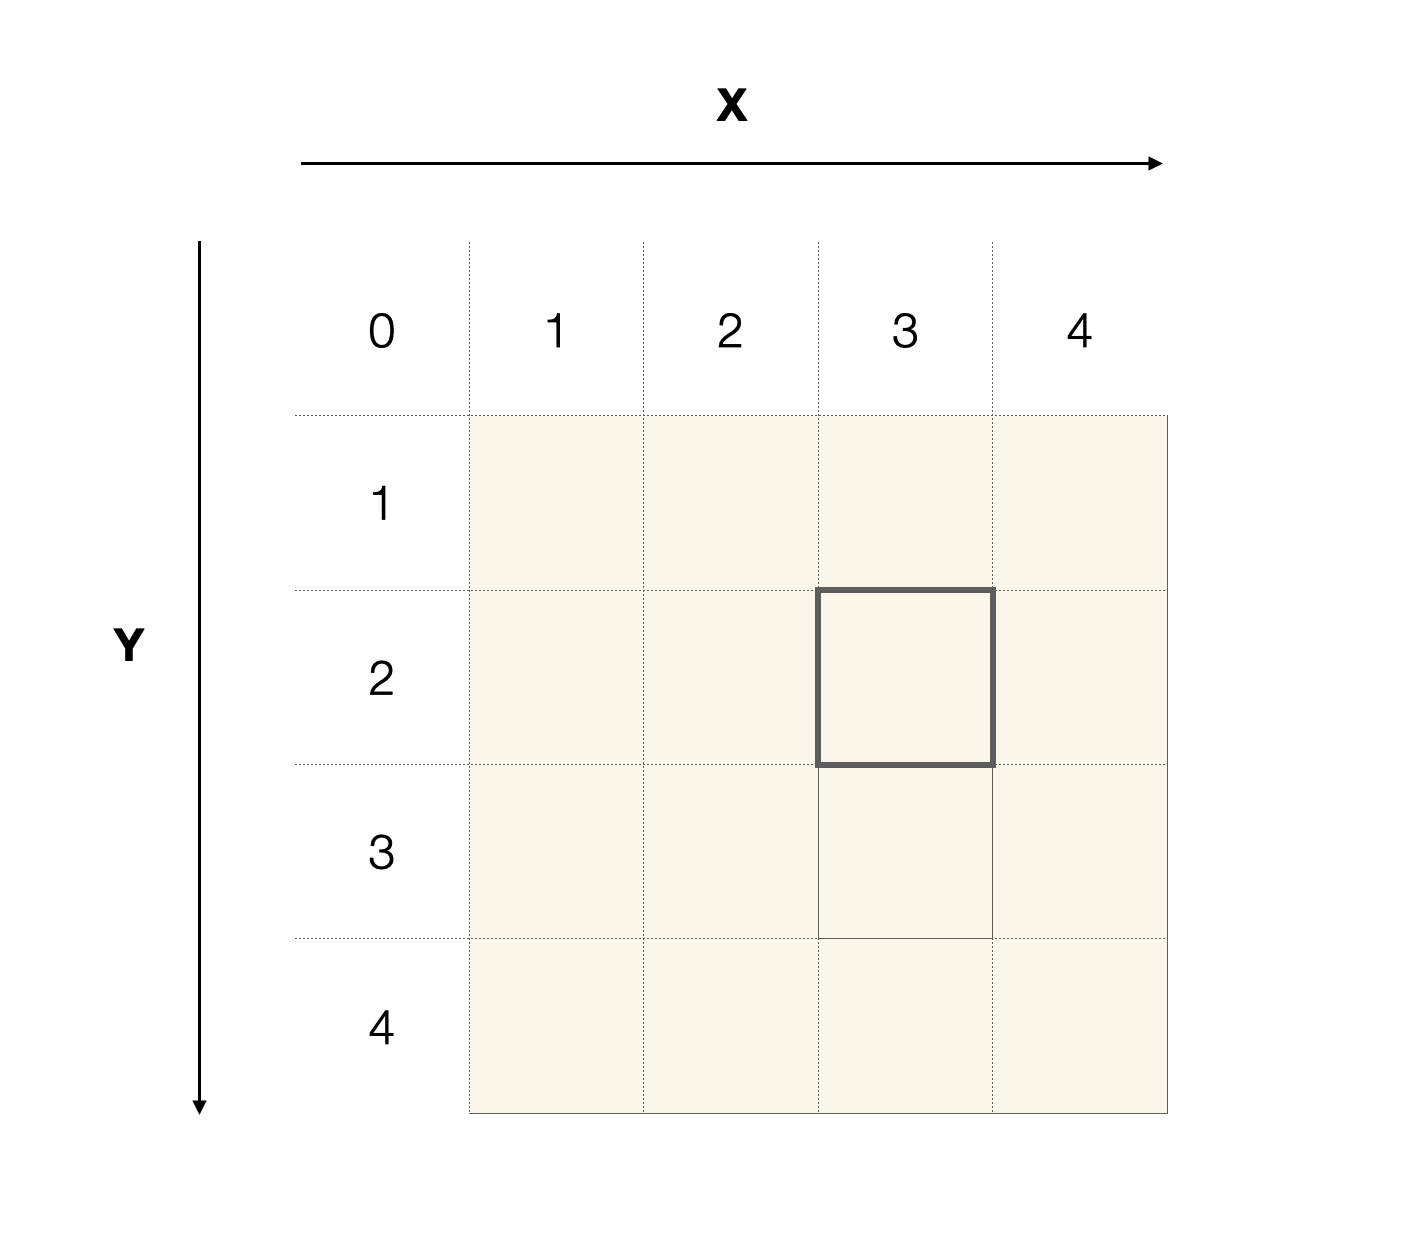
\includegraphics[scale=0.2]{pixel_coordinates}	
\end{center}
	\begin{lstlisting}
myImage.GetPixel(3, 2);
	\end{lstlisting}
	We can use the method to discover the ARGB values at the above position

\end{frame}